%%%%%%%%%%%%%%%%%%%%%%%%%%%%%%%%%%%%%%%%%%%%%%%%%%%%%%%%%%%%%%%%%%%%%%%%%%%%%%%%
%2345678901234567890123456789012345678901234567890123456789012345678901234567890
%        1         2         3         4         5         6         7         8

\documentclass{sage}

% Subfiles package
\usepackage{subfiles}

% Usual setup packages
\usepackage{listings} % For including source code with highlighting
\usepackage{hyperref} % For better hyper-link integration
\usepackage[bottom]{footmisc} % places footnotes at page bottom

% Packages for verbatim text blocks
\usepackage{alltt} % Package for including math in verbatim text
\usepackage{fancyvrb}

% Packages for math symbols and other mathey things
\usepackage{amsthm}
\usepackage{amsmath}
\usepackage{amsfonts}
\usepackage{amssymb}

% Packages for including pseudo-code
\usepackage{algorithmicx}
\usepackage{algorithm}
\usepackage{algpseudocode}

% Packages that handle tables, figures and other floats
\usepackage{tabularx}
\usepackage{multirow}
\usepackage{float} % To make floats movable
\usepackage{subcaption}
\usepackage[table]{xcolor}

% Packages for drawing graphs, FSMs, etc.
\usepackage{pgf}
\usepackage{tikz}
\usetikzlibrary{shapes,arrows,calc,fit,positioning,shapes.symbols,shapes.callouts,patterns,automata,matrix}

% Remove red boxes around refs
\hypersetup{
    colorlinks,
    citecolor=black,
    filecolor=black,
    linkcolor=black,
    urlcolor=blue
}

% ------------------------------ CUSTOM MACROS ------------------------------------
% Nice little macro for adding a comment box. Include incrementing comment numbers.
\newcounter{comcount}
\setcounter{comcount}{0}
\newcommand{\mycomment}[1]
{
\refstepcounter{comcount}
\smallskip\noindent\fbox{\parbox{\linewidth}{\emph{Comment \arabic{comcount}} : \small{#1}}} 
}

\DeclareMathOperator*{\argmin}{\arg\!\min\>}
\newcommand{\amin}[1]{\underset{#1}\argmin}
\DeclareMathOperator*{\argmax}{\arg\!\min\>}
\newcommand{\amax}[1]{\underset{#1}\argmax}

\newcommand{\sig}{\mathcal{S}}
\newcommand{\ceil}[1]{\lceil#1\rceil}
\newcommand{\xm}{x_{\hat{m}}}

%%%Article information%%%%%%%%%%%%%%%%%%%%%%%%%%%%%%%%
\journal{International Journal of Robotics Research}
\volume{000}
\issue{00}
\copyrightline{$\copyright$ Copyright}
\firstpage{1}
\lastpage{13}
\doi{doi number}
\articletype{Article type}
\pubyear{2015}
%%%%%%%%%%%%%%Article information%%%%%%%%%%%%%%%%%%%%%%%%

\begin{document}
\title{Maximizing Swarm System Utility for Time-Varying Tasks}
\author{Anshul Kanakia and Nikolaus Correll}
\address{Department of Computer Science,
	University of Colorado, Boulder, USA}

\maketitle

%%%%%%%%%%%%%%%%%%%%%%%%%%%%%%%%%%%%%%%%%%%%%%%%%%%%%%%%%%%%%%%%%%%%%%%%%%%%%%%%
\begin{abstract}
Abstract goes here\ldots
\end{abstract}
\keywords{Swarm Robotics, Multi-Agent Systems, Collaboration, Task Allocation, Utility Theory, Optimization}

%%%%%%%%%%%%%%%%%%%%%%%%%%%%%%%%%%%%%%%%%%%%%%%%%%%%%%%%%%%%%%%%%%%%%%%%%%%%%%%%
\section{Introduction}
There has been considerable research done using swarm robot systems to tackle tasks  such as firefighting. Time often plays an important role in such situations, e.g. fires tend to spread at an exponential rate if not contained quickly. Thus, the overall utility of the system also varies with time. We describe a process that maximizes time-varying utility of a swarm robot system for accomplishing time-varying tasks, through the use of sigmoid threshold functions for collaboration decisions.

The goal of this model is to represent tasks that have the property of ``concurrent benefit''. We define concurrent benefit as an attribute of a collaborative task wherein the exact number of robots required to successfully complete the task is unknown and varies with time but the probability of success depends, non-linearly, on the average number of agents assigned to that task. For example, in a firefighting scenario a single robot trying to contain a large fire will almost definitely be unsuccessful on its own (and will waste water in trying) but a group of robots within a certain group size range may be able to contain the flames to a reasonable level of success. This measure of success is related non-linearly to the group size, i.e. where 5 or even 10 robots have a negligible effect on containing the fire, perhaps 12 or more very quickly become capable of succeeding in the task. The group size to payoff ratio is described by a utility function that is itself sigmoid in nature, as seen in Fig. \ref{fig:sigmoid}.

\begin{figure}[!ht]
\centering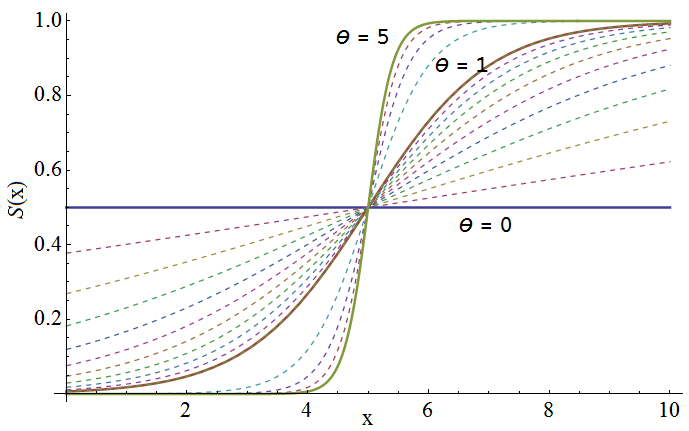
\includegraphics[width=.5\textwidth]{../figures/sigmoid1.png}
\centering\caption{}\label{fig:sigmoid}
\end{figure}



\begin{figure}[!ht]
\centering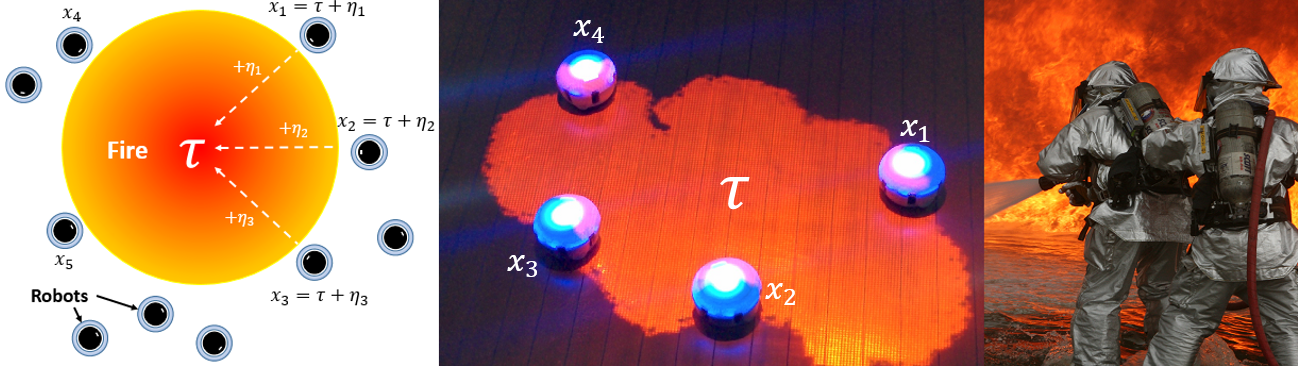
\includegraphics[width=\textwidth]{../figures/dropletfire.png}
\centering\caption{}\label{fig:dropletfire}
\end{figure}

It is for such tasks that we create this swarm system model and describe optimization methods for global, system level utility. The scenario is set up as follows. We assume a large operational area, compared to the size of a collaboration site. Collaboration sites are distributed randomly (but not necessarily uniformly) around the operational area. We assume a large swarm of robots is also dispersed in the operational area. The total number of robots is arbitrary but we assume it is unchanging throughout the course of the scenario. This is done mostly for mathematical simplicity of the system model and we later discuss how to relax this condition for size varying swarms. Each collaboration site comprises of some arbitrary task that a group of robots must perform to increase the overall system utility of the swarm. These tasks can include the aforementioned fire containment or lifting an object for collective transport, etc. Henceforth, we will use the terms collaboration site and task interchangeably.



\section{System Model}
We define the following terms for our model:
\begin{itemize}
	\item $N$   -- Total number of agents
	\item $M$   -- Total number of tasks/collaboration sites
	\item $N_i$ -- Number of agents at site-$i$
%	\item $collab(\hat{N}_i^j, \theta_i, \tau_i)$ -- Agent specific sigmoid threshold collaboration function
%	\begin{equation}
%		collab(\hat{N}_i^j, \theta_i, \tau_i) = \frac{1}{1 + e^{\theta_i\left(\tau_i - \hat{N}_i^j\right)}}
%	\end{equation}
%	\item $\hat{N}_i^j$ -- Agent-$j$'s estimate of the current number of robots at its site-$i$
%	\item $\theta_i$ -- Site specific sigmoid model variance parameter
%	\item $\tau_i$   -- Site specific sigmoid model mean parameter
	\item $R_i$ -- Agent specific resource cost of attempting task-$i$
	\item $P_i$ -- Agent specific payoff for successfully completing task-$i$
%	\item $D_i$ -- Indicator variable; $1$ if a group of agents decide to collaborate at site-$i$
	\item $D_j^i$ -- Agent specific binary decision variable indicating whether or not agent-$j$ performs task-$i$
%	\item $C_i$ -- Indicator variable; $1$ if the task at site-$i$ has been successfully completed
%	\item $k$   -- Constant cost incurred per time step at task-$i$
	\item $U_j^i$ -- Agent specific total utility time given agent-$j$ is at site-$i$
%	\begin{equation}
%		U_i(t) = -k.t.(1 - C_i) - N_i.R_i.D_i(t-1) + N_i.P_i.D_i(t-1).C_i
%	\end{equation}
\end{itemize}


The total system level ensemble utility at time-$t$ is then,
\begin{equation}
	U(t) = \sum\limits_{\forall j \in N}\sum\limits_{\forall i \in M} U_j^i(t)
\end{equation}

The objective of the system is to complete all the tasks in the environment while maximizing system utility, $U$, by tuning available agent-level parameters, i.e. $goal = \amin{\theta_i, \tau_i} U$.

%\subfile{StateMachineTikZ.tex}
%
%\section{Robot Experiments}


%%%%%%%%%%%%%%%%%%%%%%%%%%%%%%%%%%%%%%%%%%%%%%%%%%%%%%%%%%%%%%%%%%%%%%%%%%%%%%%%
%%%%%%%%%   The Bibliography, if any   %%%%%%%%%
\bibliographystyle{harvard}		% or "siam", or "alpha", etc.
%\nocite{*}						% list all refs in database, cited or not
\bibliography{../refworks}
\end{document}